
\definecolor{c0000ff}{RGB}{0,0,255}
\definecolor{cff0000}{RGB}{255,0,0}
\usetikzlibrary{arrows}

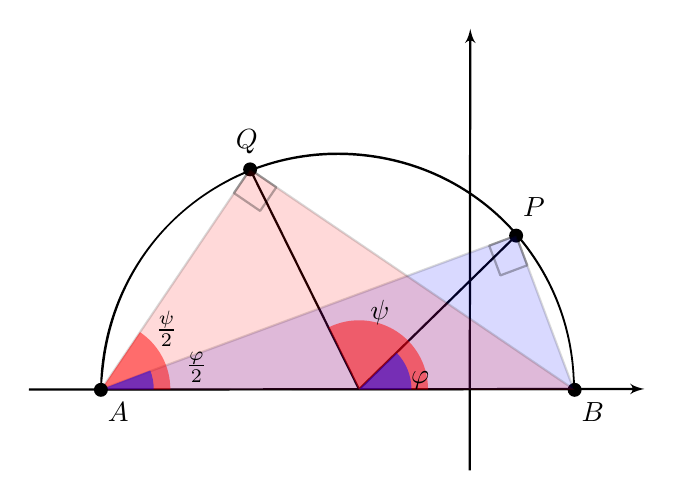
\begin{tikzpicture}[y=0.80pt, x=0.8pt,yscale=-1,scale=0.5, inner sep=0pt, outer sep=0pt]
\begin{scope}[shift={(-152.24647,-317.69709)}]% layer1
  \begin{scope}[shift={(3051.4825,-2552.5587)}]% g2090
    % path2136
    \path[draw=black,line join=miter,line cap=butt,line width=0.800pt,-latex']
      (-2899.2355,3196.2122) -- (-2343.0818,3195.6182);

    % path2138
    \path[draw=black,line join=miter,line cap=butt,line width=0.800pt,-latex']
      (-2500.9667,3269.2615) -- (-2500.3969,2870.2565);

    % path2150
    \path[cm={{0.82575,0.0,0.0,-0.82575,(-129.59075,4772.4814)}},color=black,fill=black,line
      width=0.800pt] (-3275.1575,1929.8205) .. controls (-3272.6894,1957.3643) and
      (-3265.9839,1984.5141) .. (-3255.1425,2009.9408) .. controls
      (-3242.0491,2040.6458) and (-3222.9907,2068.8007) .. (-3199.3033,2092.3240) ..
      controls (-3199.3033,2092.3240) and (-3199.3033,2092.3240) ..
      (-3199.3033,2092.3241) .. controls (-3196.4103,2095.1970) and
      (-3193.4485,2098.0006) .. (-3190.4217,2100.7317) .. controls
      (-3168.6890,2120.3413) and (-3143.7349,2136.3849) .. (-3116.7790,2147.8299) ..
      controls (-3084.9683,2161.3350) and (-3050.3963,2168.3422) ..
      (-3015.8189,2168.2784) .. controls (-3015.8189,2168.2784) and
      (-3015.8189,2168.2784) .. (-3015.8188,2168.2784) .. controls
      (-3014.5354,2168.2784) and (-3013.2520,2168.2644) .. (-3011.9688,2168.2424) ..
      controls (-2978.6867,2167.6762) and (-2945.4841,2160.9886) ..
      (-2914.7105,2148.1805) .. controls (-2885.2450,2135.9154) and
      (-2858.0563,2118.0897) .. (-2835.1556,2095.8335) .. controls
      (-2834.0856,2094.7935) and (-2833.0245,2093.7443) .. (-2831.9727,2092.6861) ..
      controls (-2831.9727,2092.6861) and (-2831.9727,2092.6860) ..
      (-2831.9727,2092.6860) .. controls (-2808.3976,2068.9665) and
      (-2789.4599,2040.6911) .. (-2776.6010,2009.8963) .. controls
      (-2764.9339,1981.9527) and (-2758.3364,1951.9686) .. (-2757.0287,1921.8072) ..
      controls (-2756.5734,1917.3341) and (-2756.5896,1914.0291) ..
      (-2756.7880,1911.8819) .. controls (-2756.9863,1909.7347) and
      (-2757.3672,1908.7418) .. (-2757.7360,1908.8475) .. controls
      (-2758.1048,1908.9533) and (-2758.4624,1910.1551) .. (-2758.6982,1912.3990) ..
      controls (-2758.9339,1914.6428) and (-2759.0483,1917.9268) ..
      (-2759.0029,1922.2309) .. controls (-2760.4135,1951.9864) and
      (-2767.0131,1981.5406) .. (-2778.5723,2009.0625) .. controls
      (-2791.3857,2039.5731) and (-2810.2242,2067.5697) .. (-2833.6318,2091.0269) ..
      controls (-2833.6318,2091.0269) and (-2833.6318,2091.0269) ..
      (-2833.6318,2091.0269) .. controls (-2834.3822,2091.7789) and
      (-2835.1372,2092.5262) .. (-2835.8969,2093.2687) .. controls
      (-2858.8246,2115.6803) and (-2886.1286,2133.5847) .. (-2915.7055,2145.8282) ..
      controls (-2945.2555,2158.0619) and (-2977.0525,2164.6041) ..
      (-3008.9626,2165.4804) .. controls (-3011.2401,2165.5434) and
      (-3013.5259,2165.5764) .. (-3015.8188,2165.5794) .. controls
      (-3032.4616,2165.6014) and (-3049.4865,2164.0242) .. (-3066.3551,2160.7364) ..
      controls (-3083.2236,2157.4486) and (-3099.9303,2152.4501) ..
      (-3115.9176,2145.7939) .. controls (-3129.7045,2140.0545) and
      (-3142.9519,2133.0999) .. (-3155.3778,2125.1595) .. controls
      (-3167.8037,2117.2190) and (-3179.4060,2108.2943) .. (-3189.9701,2098.6776) ..
      controls (-3192.7197,2096.1746) and (-3195.3971,2093.6224) ..
      (-3198.0028,2091.0242) .. controls (-3198.0028,2091.0242) and
      (-3198.0028,2091.0242) .. (-3198.0028,2091.0242) .. controls
      (-3210.0648,2078.9970) and (-3220.5978,2065.9980) .. (-3229.7148,2052.2709) ..
      controls (-3238.8319,2038.5438) and (-3246.5375,2024.0841) ..
      (-3252.8469,2008.9704) .. controls (-3257.5845,1997.6231) and
      (-3261.5238,1985.9048) .. (-3264.6712,1973.8324) .. controls
      (-3267.8187,1961.7600) and (-3270.1751,1949.3321) .. (-3271.6857,1936.5521) ..
      controls (-3271.9629,1934.3114) and (-3272.2907,1931.6065) ..
      (-3272.6070,1928.7698) .. controls (-3272.9233,1925.9331) and
      (-3273.2274,1922.9646) .. (-3273.4985,1920.2021) .. controls
      (-3274.0407,1914.6772) and (-3274.4432,1909.9732) .. (-3274.9023,1908.8402) ..
      controls (-3275.0375,1908.5067) and (-3275.1781,1908.4830) ..
      (-3275.3233,1908.8402) .. controls (-3275.3233,1908.8402) and
      (-3275.3233,1908.8402) .. (-3275.3233,1908.8402) .. controls
      (-3275.4627,1909.1829) and (-3275.6065,1909.8763) .. (-3275.7445,1910.9839) ..
      controls (-3275.8931,1913.7528) and (-3275.8877,1916.9070) ..
      (-3275.7695,1920.1457) .. controls (-3275.6510,1923.3838) and
      (-3275.4194,1926.7064) .. (-3275.1575,1929.8205) -- cycle;

    \begin{scope}[shift={(128.03018,71.58882)}]% g2179
      % path2146
      \path[shift={(-1295.4547,1536.4384)},fill=black,nonzero rule]
        (-1285.2569,1449.0822) .. controls (-1285.2569,1452.5629) and
        (-1288.0786,1455.3846) .. (-1291.5593,1455.3846) .. controls
        (-1295.0401,1455.3846) and (-1297.8618,1452.5629) .. (-1297.8618,1449.0822) ..
        controls (-1297.8618,1445.6014) and (-1295.0401,1442.7797) ..
        (-1291.5593,1442.7797) .. controls (-1288.0786,1442.7797) and
        (-1285.2569,1445.6014) .. (-1285.2569,1449.0822) -- cycle;

      % text2154
      \path[fill=black] (-2580.7356,2968.0764) node[above right] (text2154) {$P$};

    \end{scope}
    \begin{scope}[shift={(-129.74541,14.21761)}]% g2179-7
      \begin{scope}% g2215
        % path2146-4
        \path[shift={(-1277.9852,1533.9696)},fill=black,nonzero rule]
          (-1285.2569,1449.0822) .. controls (-1285.2569,1452.5629) and
          (-1288.0786,1455.3846) .. (-1291.5593,1455.3846) .. controls
          (-1295.0401,1455.3846) and (-1297.8618,1452.5629) .. (-1297.8618,1449.0822) ..
          controls (-1297.8618,1445.6014) and (-1295.0401,1442.7797) ..
          (-1291.5593,1442.7797) .. controls (-1288.0786,1442.7797) and
          (-1285.2569,1445.6014) .. (-1285.2569,1449.0822) -- cycle;

        % text2154-2
        \path[fill=black] (-2582.4631,2969.4089) node[above right] (text2154-2) {$Q$};

      \end{scope}
    \end{scope}
    \begin{scope}[shift={(2.0,0)}]% g2238
      % path2146-9
      \path[shift={(-1116.5677,1747.3139)},fill=black,nonzero rule]
        (-1285.2569,1449.0822) .. controls (-1285.2569,1452.5629) and
        (-1288.0786,1455.3846) .. (-1291.5593,1455.3846) .. controls
        (-1295.0401,1455.3846) and (-1297.8618,1452.5629) .. (-1297.8618,1449.0822) ..
        controls (-1297.8618,1445.6014) and (-1295.0401,1442.7797) ..
        (-1291.5593,1442.7797) .. controls (-1288.0786,1442.7797) and
        (-1285.2569,1445.6014) .. (-1285.2569,1449.0822) -- cycle;

      % text2154-1
      \path[fill=black] (-2401.8486,3224.9519) node[above right] (text2154-1) {$B$};

    \end{scope}
    % path1929
    \path[draw=black,line join=miter,line cap=butt,line width=0.800pt]
      (-2600.8619,3195.8935) -- (-2458.9839,3057.1093);

    % path1934
    \path[draw=black,line join=miter,line cap=butt,line width=0.800pt]
      (-2600.8619,3195.8935) -- (-2699.2899,2997.2693);

    % path1938
    \path[draw=black,fill=c0000ff,opacity=0.150,line join=miter,line cap=butt,line
      width=0.800pt] (-2834.2300,3196.1427) -- (-2458.9839,3057.1093) --
      (-2407.1557,3195.6866) -- cycle;

    % path1940
    \path[draw=black,fill=cff0000,opacity=0.150,line join=miter,line cap=butt,line
      width=0.800pt] (-2833.7991,3196.1423) -- (-2699.2899,2997.2693) --
      (-2406.1270,3196.3960) -- cycle;

    % path1946
    \path[shift={(-14.57628,176.42692)},color=black,fill=cff0000,opacity=0.500,nonzero
      rule,line width=4.320pt] (-2613.5947,2963.4748) .. controls
      (-2582.6713,2948.3924) and (-2545.3762,2961.2342) .. (-2530.2939,2992.1575) ..
      controls (-2526.1453,3000.6635) and (-2523.9891,3010.0028) ..
      (-2523.9891,3019.4666) -- (-2586.2856,3019.4666) -- cycle;

    % path1944
    \path[shift={(-14.57628,176.42692)},color=black,fill=c0000ff,opacity=0.500,nonzero
      rule,line width=4.320pt] (-2552.2550,2986.6036) .. controls
      (-2543.7378,2995.4234) and (-2538.9775,3007.2055) .. (-2538.9775,3019.4666) --
      (-2586.2856,3019.4666) -- cycle;

    % path1946-3
    \path[shift={(-247.36972,176.46328)},color=black,fill=cff0000,opacity=0.500,nonzero
      rule,line width=4.320pt] (-2551.4499,2967.8204) .. controls
      (-2534.2807,2979.4011) and (-2523.9891,2998.7569) .. (-2523.9891,3019.4666) --
      (-2586.2856,3019.4666) -- cycle;

    % path1944-0
    \path[shift={(-247.36972,176.46328)},color=black,fill=c0000ff,opacity=0.500,nonzero
      rule,line width=4.320pt] (-2542.1197,3002.5128) .. controls
      (-2540.0426,3007.9239) and (-2538.9775,3013.6705) .. (-2538.9775,3019.4666) --
      (-2586.2856,3019.4666) -- cycle;

    \begin{scope}[shift={(-425.96748,0)}]% g2238-8
      % path2146-9-4
      \path[shift={(-1116.5677,1747.3139)},fill=black,nonzero rule]
        (-1285.2569,1449.0822) .. controls (-1285.2569,1452.5629) and
        (-1288.0786,1455.3846) .. (-1291.5593,1455.3846) .. controls
        (-1295.0401,1455.3846) and (-1297.8618,1452.5629) .. (-1297.8618,1449.0822) ..
        controls (-1297.8618,1445.6014) and (-1295.0401,1442.7797) ..
        (-1291.5593,1442.7797) .. controls (-1288.0786,1442.7797) and
        (-1285.2569,1445.6014) .. (-1285.2569,1449.0822) -- cycle;

      % text2154-1-2
      \path[fill=black] (-2401.8486,3224.9519) node[above right] (text2154-1-2) {$A$};

    \end{scope}
    % rect1984
    \path[cm={{0.82536,0.5646,-0.5646,0.82536,(0.0,0.0)}},color=black,draw=black,opacity=0.300,line
      join=round,line cap=round,miter limit=4.00,dash phase=16.000pt,line
      width=0.800pt,rounded corners=0.0000cm] (-535.6256,3997.8613) rectangle
      (-506.9445,4023.7852);

    % rect1986
    \path[cm={{0.35176,0.93609,-0.93609,0.35176,(0.0,0.0)}},color=black,draw=black,opacity=0.300,line
      join=round,line cap=round,miter limit=4.00,dash phase=16.000pt,line
      width=0.800pt,rounded corners=0.0000cm] (1996.7638,3377.1963) rectangle
      (2025.4449,3403.1202);

    % text1988
    \path[fill=black] (-2553.9409,3195.8933) node[above right] (text1988) {$\varphi$};

    % text1996
    \path[fill=black] (-2590.6707,3137.3328) node[above right] (text1996) {$\psi$};

    % text2004
    \path[fill=black] (-2757.4363,3175.9297) node[above,right] (text2004)
      {$\frac{\varphi}{2}$};

    % text2008
    \path[fill=black] (-2784.7964,3157.2808) node[above right] (text2008)
      {$\frac{\psi}{2}$};

  \end{scope}
\end{scope}

\end{tikzpicture}

